\section{Selection methods at both error rates}\label{sec:methods}

A method that lowers the bar loses fewer relevant features and keeps more irrelevant ones, so methods must be compared at both error rates. E4 puts 5 relevant candidates ($\delta = 0.5$, so $s = \nmin/4$) and 5 irrelevant ones in each data set; every shadow-based method builds its own $K = 10$ shadows (one permuted copy of each candidate), and all methods see the same 240 data sets ($\nmin$ from 10 to 500, $\phat\in\{0.01, 0.1\}$, 20 repeats). \Cref{tab:methods} gives both error rates, averaged over the two prevalences, and \cref{fig:methods} shows the main methods with their uncertainty. One-shot rules share the level $1/(K+1) = 0.091$ (\cref{prop:level}); their measured false positive rates, 0.08--0.09 pooled (row P9 of \cref{tab:agreement}), make their false negative rates directly comparable.

\begin{table}[t]
\centering\small
\caption{FNR / FPR by method and minority count ($\delta = 0.5$; 300-tree XGBoost unless stated; $K = 10$ shadows; 40 data sets per entry, standard errors at most 0.05 for FNR and 0.05 for FPR). The last column is the median wall time in seconds on one core at $\nmin = 100$; Boruta-style rounds cost about 20 one-shot fits.}\label{tab:methods}
\setlength{\tabcolsep}{4pt}
\begin{tabular}{@{}lcccccr@{}}
\toprule
Method & $\nmin = 10$ & 25 & 50 & 100 & 250 & s\\
\midrule
\csname @@input\endcsname generated/table_methods 
\bottomrule
\end{tabular}
\end{table}

\begin{figure}[t]
\centering
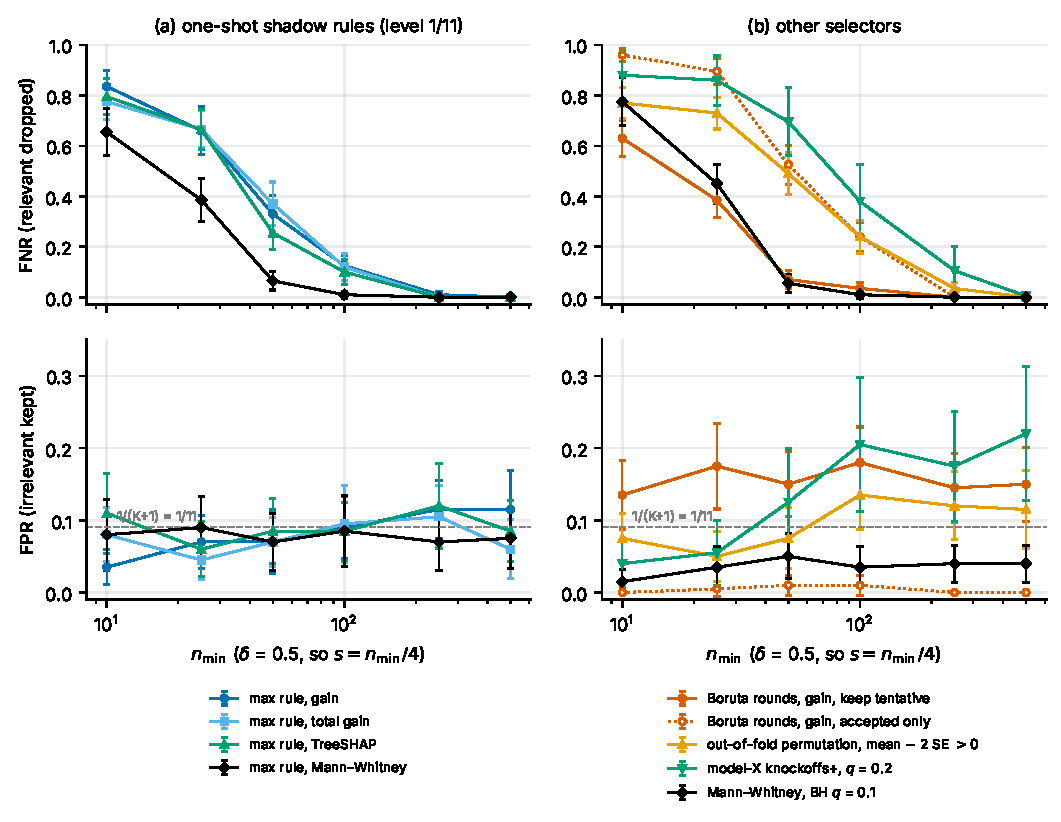
\includegraphics[width=\textwidth]{fig3_methods}
\caption{Both error rates by method ($\delta = 0.5$, the same 240 data sets for every method). Top: relevant candidates dropped; bottom: irrelevant candidates kept, with the level $1/(K+1)$ of the one-shot rules dashed. (a) One-shot max-shadow rules with three tree importances and with the Mann--Whitney statistic. (b) Other selectors. Error bars: two standard errors, clustered by data set.}\label{fig:methods}
\end{figure}

What the comparison shows:
\begin{enumerate}
  \item \emph{The importance measure matters little.} Mean gain, total gain and mean absolute TreeSHAP give the same false negative rate within two standard errors at every $\nmin$ (0.66, 0.67 and 0.67 at $\nmin = 25$). BorutaSHAP's statistic does not escape the minority-count limit.
  \item \emph{At the same level, the rank statistic loses far fewer relevant features.} With the same shadow rule, Mann--Whitney drops 0.38 of the relevant candidates at $\nmin = 25$ and 0.06 at $\nmin = 50$, against 0.66 and 0.33 for the gain. This is what \cref{cor:efficiency} and the scanning cost predict for location shifts, and the size matches \cref{prop:mw} (P13).
  \item \emph{Out-of-fold permutation importance is not more powerful.} Requiring the mean importance over five folds to exceed two standard errors keeps irrelevant candidates at the one-shot level but drops more relevant ones (0.49 at $\nmin = 50$); requiring only a positive mean keeps 0.4--0.6 of the irrelevant ones.
  \item \emph{Model-X knockoffs control false discoveries but are weak here.} With the knockoff+ threshold at $q = 0.2$ they drop 0.70 of the relevant candidates at $\nmin = 50$; the offset-free threshold has more power and an FPR near 0.3. With 10 candidates the knockoff filter has little room to work, which \cref{sec:widetables} revisits with 100 candidates.
  \item \emph{Penalised regression trades one error for the other.} Cross-validated $\ell_1$-logistic regression keeps almost every relevant candidate and 0.6--0.8 of the irrelevant ones. Stability selection with the error bound $\E V \le 1$ and threshold 0.6 selects almost nothing: with $d = 10$ candidates the bound allows only $q = \sqrt{(2\cdot 0.6-1)\,d\,\E V} \approx 1.4$ features per subsample \citep{meinshausen2010stability}, so with five relevant candidates none reaches selection probability 0.6.
  \item \emph{Boruta-style rounds help only if tentative features are kept.} Keeping tentative features drops 0.07 at $\nmin = 50$ at an FPR of about 0.15; keeping only accepted features drops 0.53 at an FPR near zero. Both match \cref{prop:rounds}: with $R = 20$ rounds, $K = 10$ and $d = 10$ the keep rate of a null candidate is about 0.10 when its hit rate does not vary, and its variation between data sets adds the rest (P12).
  \item \emph{Class weights, downsampling and early stopping do not help}, as the theory predicts: none changes $\nmin$, and downsampling the majority class to 1:1 removes information.
\end{enumerate}

% BorutaPy and the wide-table experiment (E4c, E4w) follow once the runs finish.
\subsection{Wide tables}\label{sec:widetables}

\subsection{Departures from the Gaussian model}\label{sec:robustness}

\subsection{Real data}\label{sec:realdata}
